%
% MpLtX --- a LaTeX Template for Modern Physics Lab
% Copyright (C) 2013 Modern Phys. Lab, School of Phys., Peking Univ.
%
%   MpLtX is a template for experiment report of Modern Physics Lab in
% Peking University. This template depends on the "revtex4.1" package from
% APS Journals <http://publish.aps.org/revtex/revtex-faq>
%
% To use this template, you should open the package download from APS Journals'
% website as above and follow instructions from the README file in the package.
%
% LaTeX is marvelous for math formulae composition. However, the script grammar
% is rather difficult to handle. Maybe at the beginning, it's convenient to
% generate a pretty document. The deeper you went, more weird grammar you got.
% Before you found out the whole fantesy-like world built by Knuth, Lamport and
% numerous contributors, you would get numerous strange errors unclearly
% reported by compiler.
%
% Anyway, a lot of people wish to find a general document system which is both
% easy to use and strong enough to conveniently DIY. Word is easy to use.
% However, Word can not produce perfect document in art --- the position and
% size are not well calculated. By the way, it's such a pain to do simple but
% repeating work in Word such as formating title, generate large data table
% and etc. These works can be easily done in LaTeX if you know a little about
% programming. HTML is a easy-to-use language to create static document. It is
% compatible on all the machines currently because all you need is a simple
% browser (Firefox, Chrome or IE). In HTML5, the latest version of HTML, you
% can do colorful presentation about the report. You can present dynamic
% figures to present your idea clearly. However, the biggest problem for HTML
% is that this never renders a beautiful math formula in a simple way. HTML
% indeed has a math engine named as MathML. But this guy is notorious for its
% unreadable script grammar. So HTML+TeX --- the project MathJax, becomes a
% candidate of our dream communication media or e-document form. However, it is
% still under development. If you are interested in Java, JLaTeXMath package may
% be also a proper one since it provides a LaTeX renderer in Java.
%
% This template is modified by students in Peking University.
%   I am Sun Sibai. Cao Chuanwu shared the draft on RenRen Network. However,
% the draft did not match the requirement at all. It seems that Cao Chuanwu
% did not modified the style from package. He just put the origin content
% into LaTeX format.
%   I changed the style to satisfy the format requirement and fixed some problem
% about the incompatibility within the packages.
%
% So, if you have suggestions, please improve this template with your power. We
% will be always glad to see our work useful, popular and wonderful!
%
% This template has been tested in TeXLive 2012 with the command:
% $ xelatex mpltx.tex
% compile twice.
%
% Anyone can modify this template, but don't forget to list the previous
% developers and add yourself in.
%
% Sun Sibai <niasw@pku.edu.cn>
% Cao Chuanwu <>
%
\RequirePackage{fixltx2e} %This package in CTeX is not compatible with revtex4-1
\documentclass[aps,pre,12pt,preprint,onecolumn,showpacs,showkeys]{revtex4-1}
\usepackage{ctex}
\usepackage{setspace,dcolumn}
\usepackage{subfig}
\usepackage{hyperref}
\usepackage{graphicx,psfrag,epsfig}
\usepackage[font=small,format=plain,labelfont=bf,textfont=it,justification=raggedright,singlelinecheck=false]{caption}
\usepackage{amsmath,amsfonts,amssymb,amsthm,bm,upgreek}
\usepackage{geometry}
\usepackage[mathscr]{eucal}
%\usepackage[style=alphabetic,maxnames=4,minnames=3,maxbibnames=99]{biblatex}
%\usepackage{background} %Waterstamp package
%\SetBgContents{...的实验报告} %Waterstamp to prevent copying
%\SetBgScale{5} %Waterstamp setting
\hypersetup{colorlinks=true}
\geometry{top=2.54cm,bottom=2.54cm,left=3cm,right=3cm}
\renewcommand\appendixname{附录}
\renewcommand\abstractname{摘要}
\renewcommand\tablename{表}
\renewcommand\figurename{图}
\makeatletter
\def\@pacs@name{\songti\zihao{-4}{\bf PACS码:}}
\def\@keys@name{\songti\zihao{-4}{\bf 关键词:}}
\def\Dated@name{日期:}
\def\Received@name{\zihao{-5}{接收} }
\def\Revised@name{\zihao{-5}{修订} }
\def\Accepted@name{\zihao{-5}{采纳} }
\def\Published@name{\zihao{-5}{发表} }
\makeatother
%\linespread{1}
\renewcommand{\labelenumi}{\alph{enumi}.}
\leftmargini=20mm

\begin{document}
\title{\songti\zihao{-2}\bf{机器学习在物理中的应用}\vspace{15mm}}
\author{\songti\zihao{4}北京大学物理学院2016级~~~~方永康\vspace{2mm}\\
\songti\zihao{4}北京大学物理学院2016级~~~~钱思天\vspace{2mm}}
\keywords{机器学习,神经网络,夸克-胶子等离子体,集体流}
%\email{email@pku.edu.cn; (86)152XXXXXXXX}

\begin{abstract}
\vspace{10mm}
\begin{spacing}{1.5}
\songti\zihao{-4}
本文首先介绍机器学习的概况,并且介绍了本文所用到的机器学习的方法,
包括监督式学习的神经网络(Artificial Neural Network)方法以及非监督式学习的主成分分析方法(Principal Component Analysis,PCA),贝叶斯展开(Bayesian Unfolding)。
之后介绍了在重离子碰撞领域内的研究课题,包括利用流系数以及二粒子关联函数分析重离子碰撞后产生的各向异性流,
重离子碰撞演化方程,STAR探测器时间投影室以及重离子碰撞中的长程关联行为。之后介绍了将机器学习的方法应用到这些课题中,包括在二粒子关联作为输入的情况下,
利用主成分分析以及神经网络的方法对是否存在各向异性流进行判断,利用神经网络对重离子碰撞演化方程进行拟合,利用神经网络完成探测器效率修正以及利用贝叶斯展开研究重离子碰撞长程关联行为。最终发现,
在训练数据足够充分的情况下,神经网络能够很好的区分出流事件与非流事件,并且利用PCA这一方法,
我们也发现机器能够找出流与非流事件之间的区别,而这也很有可能就是神经网络用于区分流与非流的依据;同时,神经网络可以对重离子碰撞方程给出快速的较好的拟合,并且能够对探测器机进行一定的效率修正;利用贝叶斯展开,能够对重离子
碰撞中的长程关联行为进行一定的还原。
\end{spacing}
\end{abstract}
\maketitle


\section{引言}
\subsection{机器学习简介}
近年来,随着机器学习的不断发展,其在很多领域显示出了自己强大的能力,例如在围棋上alphago战胜世界冠军李世石,在自动驾驶上逐渐发挥出巨大的作用等等。在物理方面,机器学习也显示出了它强大的能力,
例如利用PCA分析XY模型,从而使得机器能够自动区分相变\cite{PhysRevB.96.144432},
利用卷积神经网络(CNN)对粒子喷注(jet)图像进行分类\cite{PhysRevD.94.112002},利用神经网络求解薛定谔方程\cite{PhysRevA.96.042113}。
本文所采用的机器学习方法有两种,一种是使用监督式学习思想的神经网络方法,一种是使用非监督式学习思想的主成分分析方法。
\par
对于神经网络方法,它是模仿生物的神经网络传播结构而创造出来的
。其基本结构为神经元、激活函数以及损失函数。通过设计不同的神
经元以及神经元间的连接结构,在选取合适的激活函数与损失函数搭
建成合适的神经网络,再用正确的数据、正确的方法训练这一神经网
络,人们就可以得到所寻求的数据间的映射关系。人工神经网络的优
势主要体现在两方面,其一是结构中存在巨大的自由度(即存在很多
参数),其二是引入的非线性结构,因此神经网络很适合用于解决拥
有复杂映射结构的问题。但反过来说,也正是由于这两点,使得神经
网络的可解释性被削弱。
\par
而对于主成分分析方法,首先要指出我们的数据是存在于一个高维空间内的,并且数据在给定的同时,也给定了一组坐标基,主成分分析方法就是利用正交变换得到新的坐标基,使得数据在新的坐标基的方向上能够有最大的差异性(即最大的方差),从而找到决定数据之间差异的本征模式。主成分分析的优点在于所用到的变换仅仅为线性变换,因此可解释性很强。但反过来,也正是由于这一点,使得其可能无法简单的用于特别复杂的问题之中。
\subsection{重离子碰撞问题简介}
在高能物理的领域中,相对论性重离子碰撞提供了
高能量密度的环境,一般认为,在这种环境中,夸克、胶子
会解除禁闭,形成一种新的相:夸克-胶子等离子体
(quark-gluon plasma, QGP)。而想要研究QGP,就
需要能够观察到稳定的QGP信号。但由于实验中可能产生
的QGP存在时间极短、空间尺度极小以及温度极高等特点,
因此直接观测QGP本身是不现实的,因此实验上都是通过测
量碰撞后的产物来间接推测QGP的性质。目前发现,QGP的性
质可以用流体进行很好的模拟,这一研究方法被称为集体
流。\cite{2017arXiv170300670S}也就是说,由于QGP的性质与流体十分相似,具有很强
的集体行为,因此,碰撞后形成的QGP在能量密度上的各向
异性会体现在末态粒子在动量空间分布上的各向异性中。通
过研究末态粒子在动量空间上的分布,我们可以推知QGP的相关性质。但是,在真实的实验中,单个碰撞事件产生的末态粒子很少,因此各向异性流的信号十分微弱,其统计涨落现象十分严重,同时每次碰撞事件中还有非流效应,例如喷注(jet)、双喷注(dijet)等现象,也使得各向异性流的效应难以观测。因此实验上一般采用大量碰撞事件平均的方法抑制涨落,同时使用二粒子关联等方法去除非流效应,从而得到适合研究的流信号。但这种手段需要的事件数极其巨大,同时也不可能获得完全纯净的流信号,因此,需要一种新的方法,使得能够在较少事件平均下(甚至是逐事件下)能够高效的区分流与非流。

\section{机器学习方法} 
前面简要介绍了一下本文所用的研究方法,神经网络方法以及主成分分析方法。下面将简要介绍一下其中的细节。
\subsection{神经网络}
神经网络来源于仿生学,是模仿生物神经网络而创建的新的方法。
实现其功能的基本单元为:神经元及神经元间的连接,激活函数,损失函数。
而一般的前馈神经网络的结构如图~\ref{fig:cnn} 所示。整个网络由许多包含很多
神经元的层组成,大体可以分为输入层,隐藏层和输出层。我们将数据输入作为输入层再
通过神经元的连接传入隐藏层,隐藏层可能有多个,并且相邻的两个隐藏层之间也通过神经元
相连接起来,最终将结果传递至输出层输出。
我们用最简单的前馈神经网络的层间连接来演示神经网络神经元间的连接,
对于相连的两层,我们假定前后两层分别为
$\alpha$、$\beta$层,前后两层分别有$n_{\alpha}$、$n_{\beta}$个神经元,并且
两层存储的数据由向量$\bm h^{\alpha}$、$\bm h^{\beta}$表示,如图~\ref{fig:cjlj} 所示。
因此$\beta$层神经元的数据可由式~\ref{eq:1} 表示。
\begin{equation}
h_{j}^{\beta}=f(\sum_{i=1}^{n_{\alpha}}W_{ji}h_{i}^{\alpha}+b_{j}) \label{eq:1}
\end{equation}
其中$h_{i}^{\alpha}$、$h_{j}^{\beta}$是$\alpha$、$\beta$层存储数据的向量$\bm h^{\alpha}$、$\bm h^{\beta}$
在第$i$、$j$个神经元上的分量,$W_{ji}$为权重参数,$b_{j}$为偏置参数,这两者一般就是神经网络
需要训练的参数,$f$为前面提及的激活函数,用于引入非线性效应。这就是一般神经网络神经元之间的连接。\par
经过层层连接,最终连接至输出层,在输出层将利用损失函数来判断网络的输出与真实结果之间的差,之后通过
反向传播算法,来拟合前面提到的权重参数与偏置参数,从而是网络获得接近真实值的输出,即网络训练完成。
一般而言,神经网络用于处理回归问题与分类问题,对于两种问题所用到的损失函数一般不相同。我们假定网络输出值
为$y^{p}$,真实结果为$y^{r}$,那么对于回归问题一般用平方损失函数~\ref{eq:2} ,对于分类问题一般用交叉熵损失函数~\ref{eq:3}。
\begin{align}
Loss(y^{p},y^{r})&=\|y^{p}-y^{r}\|^{2} \label{eq:2} \\
Loss(y^{p},y^{r})&=-\sum_{i}y_{i}^{r}lny_{i}^{p} \label{eq:3}
\end{align}
\par
\begin{figure}[t]
\centering
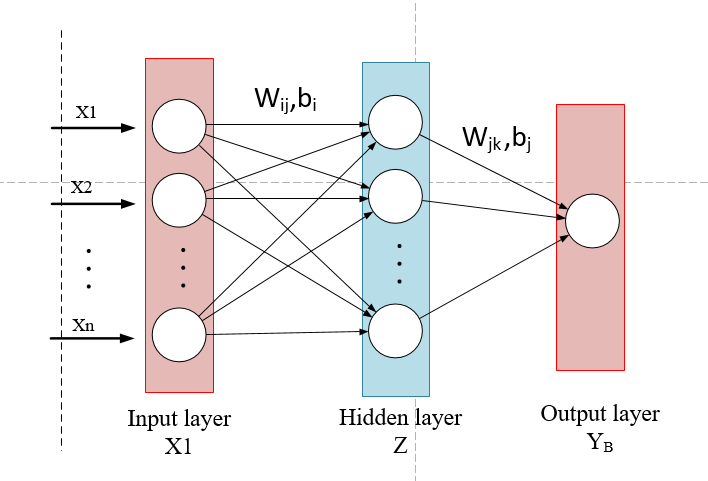
\includegraphics[width=80mm]{CNN}
\caption{\label{fig:cnn}%
此图表示了前馈神经网络的一般结构,数据从输出层输入,被传递
入隐藏层,最终通过输出层输出}
\end{figure}
\begin{figure}[t]
\centering
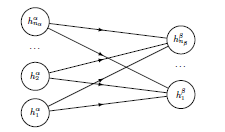
\includegraphics[width=80mm]{cjlj}
\caption{\label{fig:cjlj}%
此图表示了前馈神经网络层与层之间的联系}
\end{figure}
\begin{figure}[t]
\centering
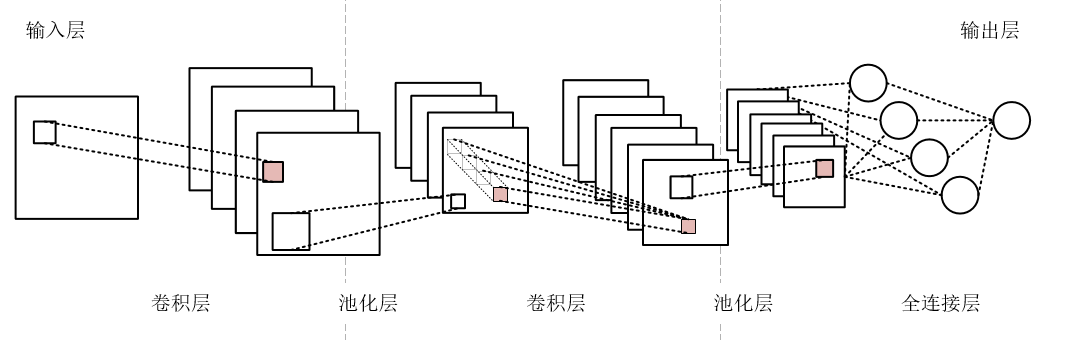
\includegraphics[width=80mm]{cnnn}
\caption{\label{fig:cnnn}%
此图表示了卷积神经网络的一般结构,其中较为特别的是卷积层与池化层}
\end{figure}
\begin{figure}[t]
\centering
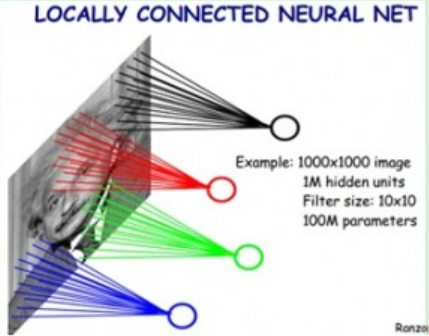
\includegraphics[width=80mm]{cnv}
\caption{\label{fig:cnv}%
此图表示了卷积层的工作模式}
\end{figure}
\begin{figure}[t]
\centering
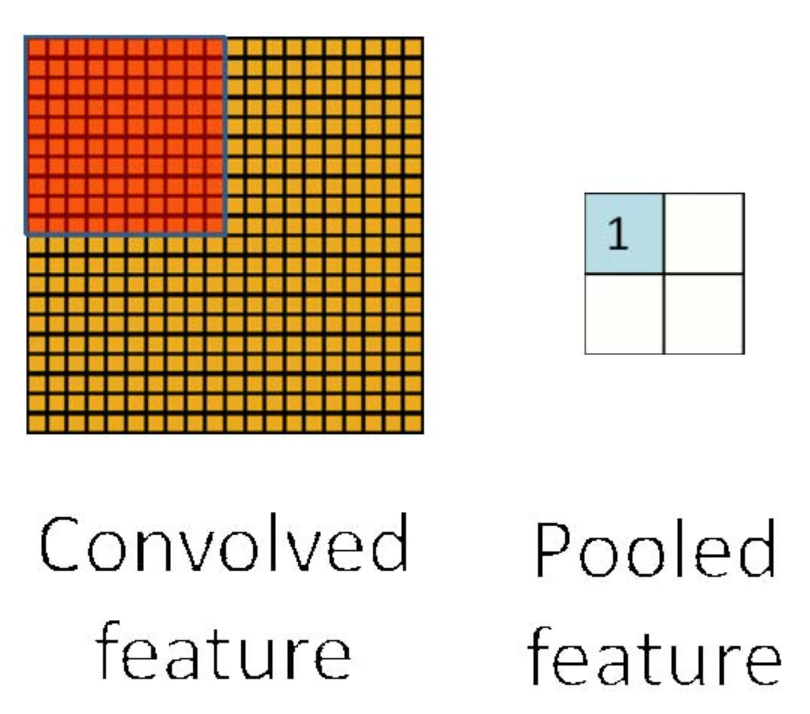
\includegraphics[width=80mm]{pool}
\caption{\label{fig:pool}%
此图表示了池化层的工作模式}
\end{figure}
本文所用到神经网络为传统的卷积神经网络(Convolutional Neural 
Network, CNN)。其基本结构如图~\ref{fig:cnnn} 所示。可以看到,与之前展示的前馈神经网络相比,二者基本一致,
只是对于卷积神经网络有两类特殊的层,即卷积层与池化层,下面将简要解释下。对于卷积层,如图~\ref{cnv} ,一个重要的思想就是共享参数。
前一层为爱因斯坦图像,后一层为四种颜色点所示的一层,这四个点
与前一层部分点相连,更合理的想法为有一个滤波器存储相关参数,其扫过前一层,按照类似前面所述的层与层间的
运算规则,会得到新一层,因此,新一层的所有神经元均通过此滤波器上的参数与前一层的部分神经元相连,因此在这两层之间实现了参数共享,
而这就是卷积层的工作原理,而此时如果选择多个滤波器,就可以得到对应于同一层的多个新层,这也就实现了多通道
,也就是图~\ref{fig:cnnn} 中所示的前后两层可能有不同的通道数。对于池化层,如图~\ref{fig:pool} 所示,
图中两层直接相连,前一层的红色区域与池化层的蓝色区域相对应,其余部分各自对应,然后对应的区域按一定的规则,例如:
仅取最大值或取平均值规则来得到下一层,得到的新层即为池化层,按所用规则对应为最大池或平均池。这两种层的优点在于,
卷积层能够提取出图像中的局部信息,池化层能够压缩数据,防止过拟合等等。
\begin{figure}[t]
\centering
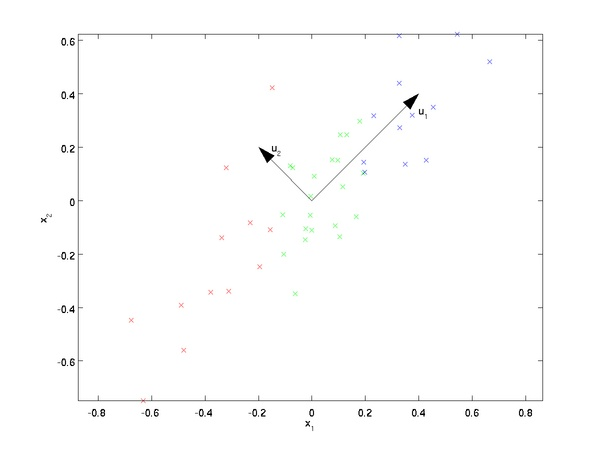
\includegraphics[width=80mm]{pca}
\caption{\label{fig:pca}%
此图表示了主成分分析的工作模式}
\end{figure}

\subsection{主成分分析}
主成分分析属于非监督式学习的范畴,下面将简要介绍一下其原理\par
首先我们指出,我们得到的所有数据都是分布在一定的高维空间之中,但是我们的数据在初始给定的
这个空间的各个基上一般是相关的,主成分分析的思路即是选择一组新的基,使得数据在这些机上一般
是相互独立的。如图~\ref{fig:pca} 所示,初始数据是分布在\{$x_{1}$,$x_{2}$\}两个基构成的二维
平面内,可以看出,数据在这两个基上的分布是高度相关的,而主成分分析即是通过一定的数学手段找到一组新的
基\{$u_{1}$,$u_{2}$\},可以看出,数据在这两个基上的分布几乎是独立的。下面将简要介绍一下如何实现这一变换。\par
假设我们的数据为$n$个$m$维数据,记为向量$\bm x_{i}$($i=1,2,\cdots,n$),这就表示$n$个具有$m$个特征的样本。
因此,我们可以得到样本的均值为:
$\bm{\bar{x}}=\sum_{i=1}^{n}\bm{x_{i}}$,之后我们可以得到数据在这$m$个特征维度上的
协方差为$Cov=\sum_{i=1}^{n}\bm{(x_{i}-\bar{x})(x_{i}-\bar{x})}^{T}$,这样得到的是一个$m*m$维的协方差矩阵,我们
可以对这个矩阵进行对角化,这样会得到一组新的基,不难理解,数据在新的基上的分布是相互独立的,并且,本征值越大,表明数据
在这个基方向上分布的差异性最大,对我们也越有意义,挑出本征值较大的几个基方向,也就是这组数据的主成分。至此,我们便实现
了主成分分析。

\begin{figure}[t]
\centering
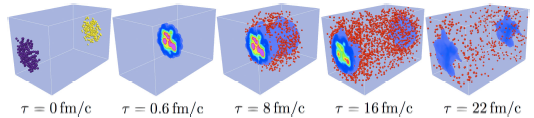
\includegraphics[width=140mm]{QGP}
\caption{\label{fig:QGP}%
此图表示了相对论性重离子碰撞产生QGP的过程}
\end{figure}
\begin{figure}[t]
\centering
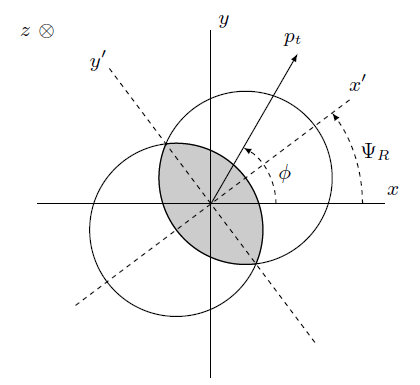
\includegraphics[width=80mm]{hz}
\caption{\label{fig:hz}%
核子相碰示意图}
\end{figure}
\section{相对论重离子碰撞}
在相对论性重离子碰撞过程中,由于其生成的高密度环境,可能使得夸克和
胶子接触禁闭,形成QGP,整个过程可由图~\ref{fig:QGP} 表示\cite{2013PhDT........31Q}。
可以看出,在碰撞后的零点几飞米时间内(除以光速不再叙述),出现QGP,在
碰撞后的几飞米时间内,会重新生成新的粒子,最终,探测器可以探测到最后的
粒子分布。为了研究QGP的性质,但受限于其存在时间极短,空间尺度极小等特点,
需要通过最终的粒子分布来间接的推知QGP的性质。现在认为,QGP的性质与流体
相似,都有很强的集体行为,而采用流体的方法来研究QGP的性质的方法即为集体流方法,
也可以称为各向异性流方法\cite{2010LanB...23..240H}。
\subsection{定义}
如图~\ref{fig:hz} 所示,表示的式在垂直粒子数方向上两核子相碰的相关物理量,
$x-y-z$为实验室坐标系,$x^{'}-y^{'}$为两核子中心连线方向坐标系,其中$x^{'}$与$x$之间
的夹角为$\psi_{R}$,被称为反应平面角(event plane angle)。$p_{t}$表示最终形成的粒子
的动量在$x-y$平面上的分量,$\phi$为$p_{t}$在$x-y$平面内的方位角,赝快度$\eta=arctanh(\frac{p_{z}}{|p|})$
用于表示粒子在$z$方向上分布性质。因此,粒子的产额可用式~\ref{eq:4} 表示\cite{PhysRevC.58.1671}。
\begin{equation}
E\frac{d^{3}N}{dp^{3}}=\frac{1}{2\pi}\frac{d^{2}N}{p_{t}dp_{t}d\eta}(1+\sum_{i=1}^{\infty}2v_{n}cos(n(\phi-\psi_{R}))) \label{eq:4}
\end{equation}
其中,傅里叶展开系数$v_{n}$用于表示各阶各向异性流的强度,其中$v_{2}$为椭圆流,$v_{3}$为三角流。通过研究
各阶流,既可以间接研究碰撞时的相关物理过程。研究各阶流的方法有很多,一般有事件平面法,二粒子和多粒子关联法,
子事件方法等。本文在研究时用到的方法是二粒子关联函数法,下面简要介绍下。
\subsection{二粒子关联函数法}
二粒子关联函数的定义如式~\ref{eq:5} 所示\citet{PhysRevC.96.024908,PhysRevLett.116.172302},其中自变量$\Delta\phi$、$\Delta\eta$分别表示两粒子的方位角$\phi$与
赝快度$\eta$的差值。同时$S(\Delta\phi,\Delta\eta)$是同一碰撞事件所有粒子对在($\Delta\phi$,$\Delta\eta$)空间
上的分布,其中包含了所有的关联,即既包含了物理上的关联,也包含了非物理的关联。而$B(\Delta\phi,\Delta\eta)$是背景
的分布,其来源于两个不同碰撞事件的粒子对在($\Delta\phi$,$\Delta\eta$)空间上的分布,其中只包含非物理的关联。同时
要考虑到涨落的影响,因此在实验上,$S(\Delta\phi,\Delta\eta)$和$B(\Delta\phi,\Delta\eta)$将进行大量事件平均后,
最终得到在事件平均下的二粒子关联函数$C(\Delta\phi,\Delta\eta)$。
\begin{equation}
C(\Delta\phi,\Delta\eta)=\frac{\sum_{events}S(\Delta\phi,\Delta\eta)}{\sum_{events}B(\Delta\phi,\Delta\eta)} \label{eq:5}
\end{equation}
\par
如图~\ref{fig:fnf} 所示\citet{PhysRevC.96.024908},左图表示的是非流事件的示意图,右图表示的是流事件的示意图。可以看到非流时间仅有在$\Delta\phi=0,\Delta\eta=0$
处的尖峰结构以及在$\Delta\phi=\pi$处的脊结构,而对于流事件,还存在$\Delta\phi=0$处的脊结构,这被称为流事件中的双脊结构,
而这也是区分流与非流事件的一个很重要的特征。
\begin{figure}[t]
\centering
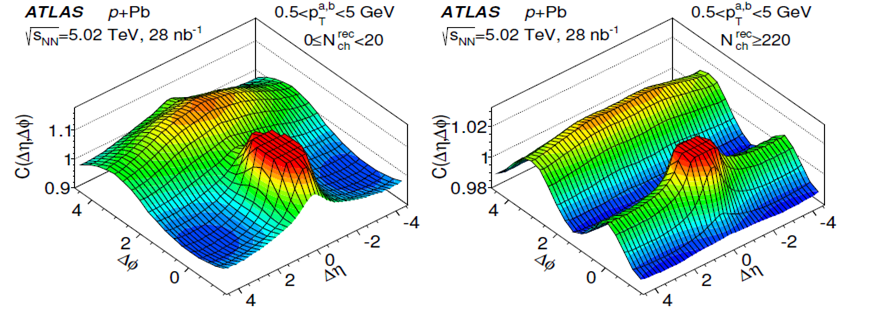
\includegraphics[width=140mm]{fnf}
\caption{\label{fig:fnf}%
流与非流的二粒子关联函数示意图,左图表示的是非流的图像,右图表示的是流的图像}
\end{figure}
\subsection{相对论性重离子碰撞的建模}
\subsubsection{逐事件约化厚度核拓扑模型(TRENTO)}
逐事件约化厚度核拓扑模型,是一个简约,计算迅速的相对论性核碰撞(质子对撞,质子重核对撞,重核对撞)初态模型。
\par
相对论性重离子碰撞领域中已经存在许多成功的初态模型,动力学模型有基于色玻璃凝聚有效场论的基于碰撞参数的Glasma模型(IP-Glasma),静态模型则有蒙特卡洛Glauber模型(MC-Glauber),都各自成功的解释了实验数据。而逐事件约化厚度核拓扑模型,则可以通过模型参数的选取,分别贴近不同的初态模型。
\par


\section{研究课题}
\subsection{利用机器学习鉴别流与非流}
\subsubsection{输入数据以及数据预处理}
我们选择的输入数据是事件平均后的二粒子关联函数,即式~\ref{eq:5} 中的$C(\Delta\phi,\Delta\eta)$。
具体而言,在计算过程中,我们首先需要计算$S(\Delta\phi,\Delta\eta)$和$B(\Delta\phi,\Delta\eta)$,
对于这两者,我们首先将$\Delta\phi\in[-0.5\pi,1.5\pi),\Delta\eta\in[-5.0,5.0)$这一区域划分为$32*32$
的各点,之后仅统计每个事件中横动量$p_{t}\in(0.5Gev/c,2.5Gev/c)$的所有带电粒子组成的粒子对在这$32*32$的
格点上的分布\cite{PhysRevC.89.064910},得到单个事件的$S(\Delta\phi,\Delta\eta)$以及两个事件的$B(\Delta\phi,\Delta\eta)$,之后将
这两者进行100个事件的平均,最终得到在100个事件平均下的二粒子关联函数$C(\Delta\phi,\Delta\eta)$。在进行归一化处理后也就得到了
我们后续处理所用到的输入数据。\par
以上介绍了我们如何获得所需要的输入数据,下面简要介绍一下数据的来源。此课题中所用到
的数据均来自于理论模型生成的数据,其中用于生成流事件的模型为Ampt与Karpenko,用于生成非流事件的
模型为Hijing和Pythia。其中Ampt模型模拟\cite{PhysRevC.72.064901}的是中心度在2030内,碰撞能量在39、100、200、500Gev的铅铅碰撞;Trento
模型模拟的是中心度在2030、3040、4050,碰撞能量为39Gev的金金碰撞;Hjing模型\cite{PhysRevD.44.3501}模拟的是在全中心度,碰撞能量为39Gev
的金金碰撞;Pythia模型模拟的是全中心度、碰撞能量为13Tev的质子质子碰撞。如图~\ref{fig:sample} 表示的为在大量事件
平均下各个模型的二粒子关联函数示意图。可以看到,用于生成流事件的Ampt与Trento模型,呈现出了明显的双峰结构,而
用于生成非流事件的Hijing和Pythia模型则没有出现双峰结构。
\begin{figure}[t]
\centering
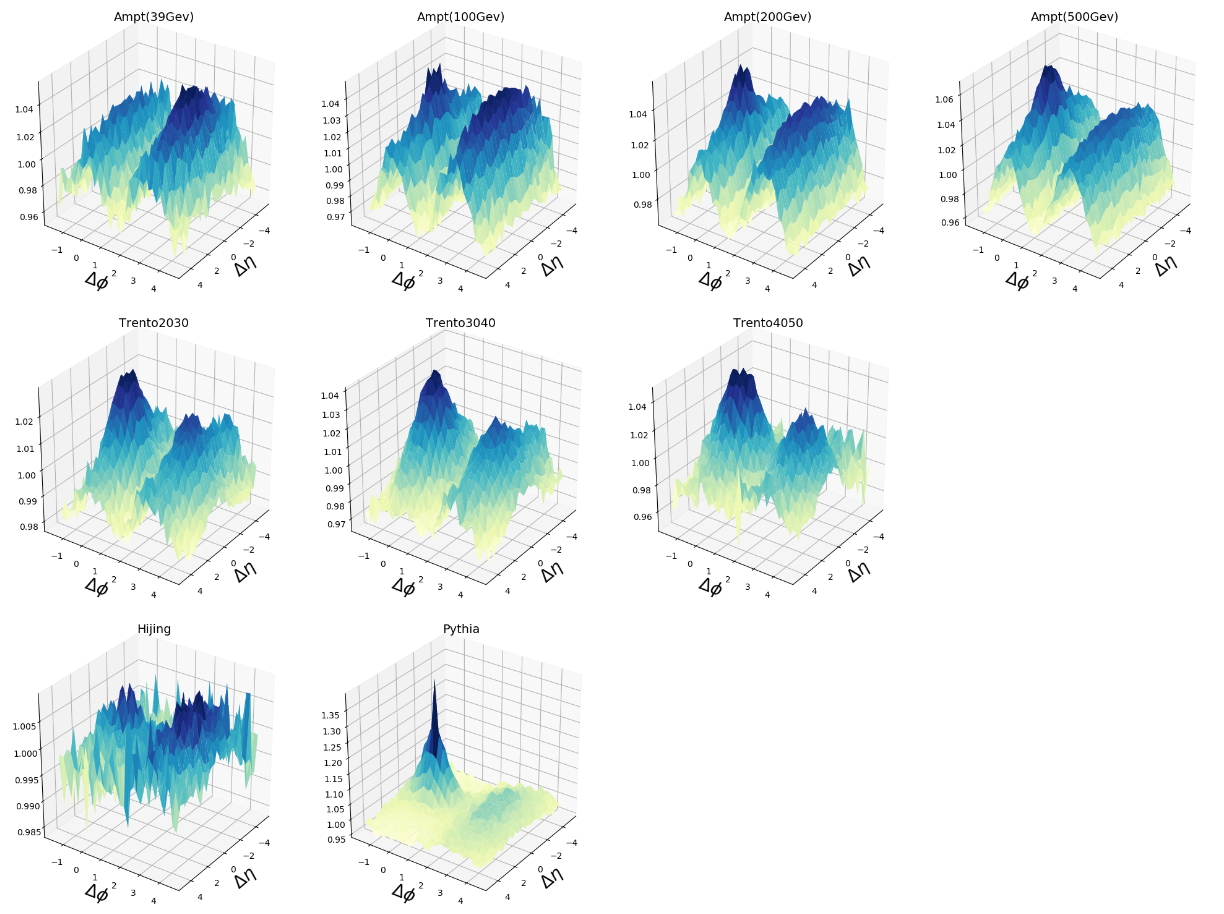
\includegraphics[width=140mm]{sample}
\caption{\label{fig:sample}%
各模型得到的二粒子关联图像示意图,各图均是在大量事件平均的基础上得到的,前两行是流事件模型,第三行是非流事件模型}
\end{figure}

\subsubsection{流与非流事件的主成分分析}
我们首先采用主成分分析的方法来对流与非流事件进行分类,需要提及的一点是,我们在用主成分分析是所用到的二粒子关联函数
并非式~\ref{eq:5} 中的$C(\Delta\phi,\Delta\eta)$,而是其中的$S(\Delta\phi,\Delta\eta)$,如图~\ref{fig:pcasample} 所示。在这里,我们使用Ampt(39Gev)、
Trento2030、Hijing三个模型进行主成分分析,得到的结果如图~\ref{fig:pcaresults} 所示。其中左图表示的是使用主成分分析找出的各个主成分对应的本征值大小,本征值越大
表明,此主成分对应的特征向量越能表示数据的性质。从左图可以看出,有两个特征值特别大,因此,这两个特征值对应的特征向量即可表示数据的大部分特征,因此做出数据在这两个特征向量
构成的平面上的分布图,如右图所示,可以发现在这两个特征向量下,数据被很好的区分开。而这两个特征向量如图~\ref{fig:tzxl} 所示,可以发现,这两个特征向量均刻画了前面提及的
流事件的双脊效应,因此,在一定程度上主成分分析找到了流与非流事件的区别。我们可以考虑将这两个特征向量进行线性组合得到流与非流事件的区别,如图~\ref{fig:qb} 所示,
黑线即是这两个特征向量进行线性组合构造的流与非流事件的分界线,黑线右上方认为是流事件,左下方认为是非流事件。
在此分界线下,用Ampt(200Gev)的数据进行测试,结果如图~\ref{fig:cs} 所示,可以看出,测试结果符合我们的预期。但是必须指出的是,此黑线的划定有很大的自由度,因此很难精确
的区分流与非流的混合事件。同时,从数据的分布可以看出,此结果具有很强的模型依赖性,而这对我们寻找流和非流的本质区别是有害的,因此我们需要其他的方法来精确的确定流与非流的本质区别,下面
我们将用神经网络进行尝试。

\begin{figure}[t]
\centering
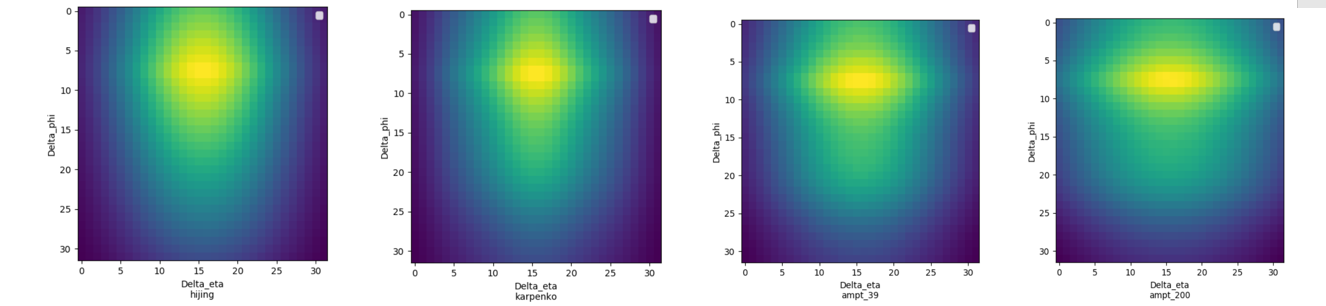
\includegraphics[width=140mm]{pcasample}
\caption{\label{fig:pcasample}%
Hijing,Trento2030\footnote{图中表示为Karpenko},Ampt(39Gev),Ampt(200Gev)在大量事件平均下$S(\Delta\phi,\Delta\eta)$的示例图}
\end{figure}
\begin{figure}[t]
\centering
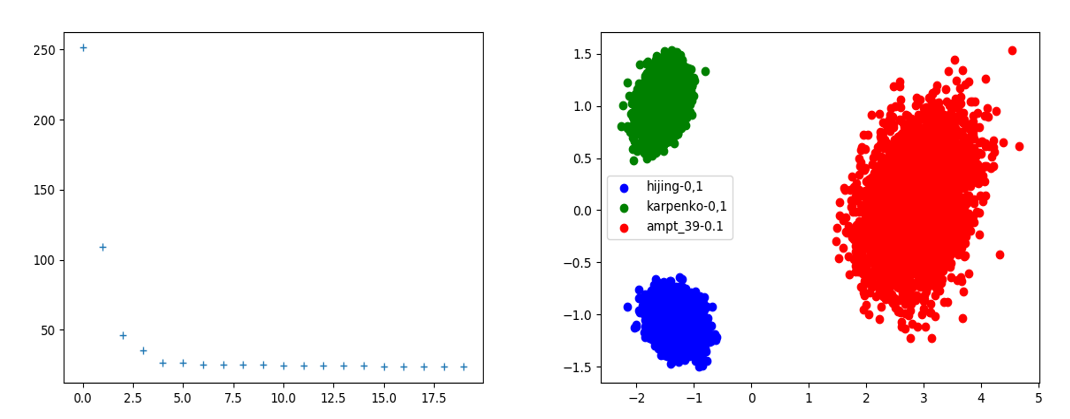
\includegraphics[width=140mm]{pcaresults}
\caption{\label{fig:pcaresults}%
对Hijing,Trento2030\footnote{图中表示为Karpenko},Ampt(39Gev)进行主成分分析得到的结果图,左图是各个特征向量对应的特征值大小,右图为输入数据在第一个和第二个
特征向量组成的平面上的分布}
\end{figure}
\begin{figure}[t]
\centering
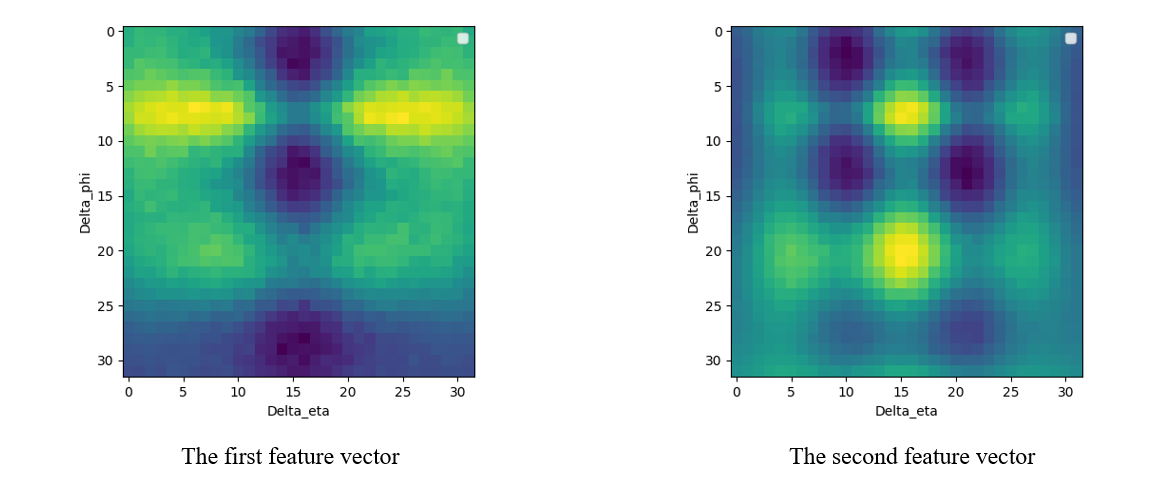
\includegraphics[width=140mm]{tzxl}
\caption{\label{fig:tzxl}%
对Hijing,Trento2030,Ampt(39Gev)进行主成分分析得到的
第一第二个特征向量,左边为第一个,右边为第二个,横坐标为$\Delta\eta$,0-32表示的是$\Delta\eta\in(-5,5)$
,纵坐标为$\Delta\phi$,0-32表示的是$\Delta\phi\in[-0.5\pi,1.5\pi)$}
\end{figure}
\begin{figure}[t]
\centering
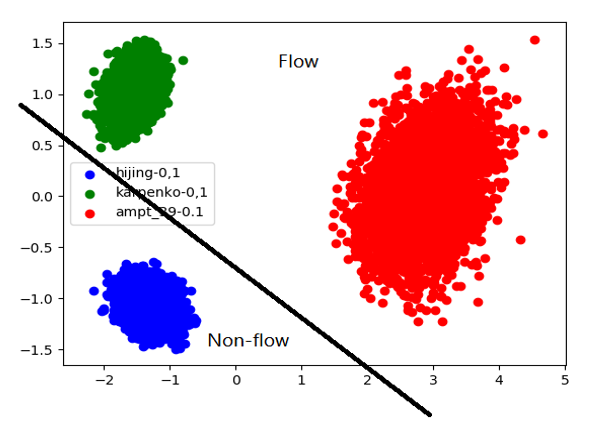
\includegraphics[width=140mm]{qb}
\caption{\label{fig:qb}%
假定的流与非流事件的分界线,即图中黑线所示}
\end{figure}
\begin{figure}[t]
\centering
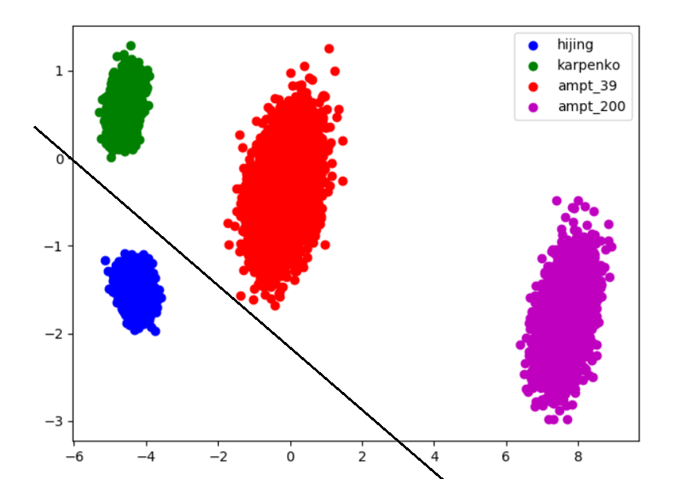
\includegraphics[width=140mm]{cs}
\caption{\label{fig:cs}%
用Ampt(200Gev)的数据测试假定的流与非流事件的分界线,即图中黑线所示}
\end{figure}

\subsubsection{流与非流事件的神经网络分类分类}
实验中所用到的卷积神经网络结构如图~\ref{fig:sjwl} 所示,同时所用到的二粒子关联函数
为式~\ref{eq:5} 中的$C(\Delta\phi,\Delta\eta)$,其样式如图~\ref{fig:sample} 所示。我们将流事件标记为(1,0),将非流事件标记为(0,1),然后
让神经网络学习从输入数据到标签的映射,最终训练好的网络将能够实现对流与非流事件的分类。
我们在输入层输入数据,然后两次经过卷积核为3*3的卷积层和最大池池化层,再展开为向量,经过两次全连接后,通过
输出层输出。在整个过程中,除输出层所用激活函数为Softmax外,其余均为Relu。所用损失函数为交叉熵损失函数。\par
训练网络时,首先我们选择仅用一个流模型与非流模型的100个事件平均后的数据各5000组作为训练集,之后用所有的模型下的100个
事件平均后的各10000组数据作为测试集来测试网络的结果,测试的准确度是指,网络输出正确标签的组数占总组数的百分比。
得到的结果如表~\ref{table:1} 所示,可以看出,仅用一种流与非流模型作为训练集的话,总会有个别模型的结果表现十分差,这表明我们的输入数据不足,使得网络
并未学到流与非流之间本质区别。\par
之后将所有流与非流模型的数据均作为训练集,
得到的结果如表~\ref{table:2} 所示,可以看出,在我们用所有的流与非流模型作为训练后,网络可以在测试集上的表现十分好,
同时我们研究了在不同事件平均下网络的表现结果,即对涨落压制在程度强弱下,网络的表现结果,可以看出,在1000、100、50个事件平均下,网络的表现都十分
良好,这表明,涨落在对于网络的分辨本领影响并不是十分巨大,只要在一定的事件数平均下,对涨落造成了一定程度上的抑制,网络
就可以得到一个比较好的表现结果。
\begin{figure}[t]
\centering
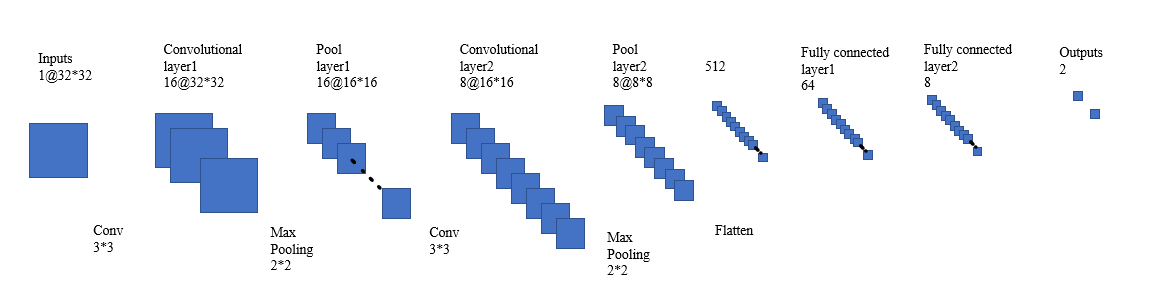
\includegraphics[width=140mm]{sjwl}
\caption{\label{fig:sjwl}%
鉴别流与非流所用到的卷积神经网络结构图}
\end{figure}

\begin{table}[t]
\caption{\label{tab:table1}%
在不同训练集训练下,测试集上网络的表现行为,所用到的所有数据都是在100个事件平均下的结果}
\begin{ruledtabular}
\begin{tabular}{lllll}
测试集 & 准确度1\footnote{此结果使用的训练集为Ampt(39Gev)、Ampt(200Gev)、Hijing}
 &准确度2\footnote{此结果使用的训练集为Ampt(39Gev)、Ampt(100Gev)、Ampt(200Gev)、Ampt(500Gev)、Pythia}
 &准确度3\footnote{此结果使用的训练集为Trento2030、Trento3040、Hijing}
 &准确度4\footnote{此结果使用的训练集为Trento2030、Pythia} \\
\colrule
Ampt(39Gev)&99.95\%&98.88\%&100\%&0\% \\
Ampt(100Gev)&98.77\%&100\% &100\%&80.08\%\\
Ampt(200Gev)&97.75\%&100\% &100\%&100\%\\
Ampt(500Gev)&99.57\%&100\% &99.57\%&100\%\\
Trento2030&4.99\%&100\% &99.59\%&100\%\\
Trento3040&58.22\%&100\% &100\%&100\%\\
Trento4050&97.89\%&100\% &100\%&99.78\%\\
Hijing&99.98\%&0\% &99.11\%&0\%\\
Pythia&0\%&100\% &0\%&100\%\\
\end{tabular}
\end{ruledtabular}
\end{table}

\begin{table}[t]
\caption{\label{tab:table2}%
在相同训练集训练,在不同数目事件平均下,测试集上网络的表现行为\footnote{所用到的训练集数据均为Ampt(39Gev)、Ampt(500Gev)、Trento3040、Hijing、Pythia}}
\begin{ruledtabular}
\begin{tabular}{llll}
测试集 & 准确度1\footnote{此结果是在1000个事件平均下的结果}
    &准确度2\footnote{此结果是在100个事件平均下的结果}
    &准确度3\footnote{此结果是在50个事件平均下的结果}\\
\colrule
Ampt(39Gev)&100\%&100\%&99.93\%\\
Ampt(100Gev)&100\%&100\% &91.82\%\\
Ampt(200Gev)&100\%&100\% &99.65\%\\
Ampt(500Gev)&100\%&100\% &100\%\\
Trento2030&99.97\%&99.99\% &99.97\%\\
Trento3040&100\%&100\% &100\%\\
Trento4050&100\%&100\% &100\%\\
Hijing&99.99\%&99.96\% &100\%\\
Pythia&100\%&100\% &100\%\\
\end{tabular}
\end{ruledtabular}
\end{table}








\section{结论}
在流与非流事件的分类课题中,我们采用了主成分分析和神经网络两种方法进行了尝试。其中主成分分析方法
可以在定性上给出流与非流事件的区别,并且能够直观的显示出流与非流事件区别的形式;而神经网络方法在训练集足够充分的情况下,能够很好的区分流与非流事件,并且只要
事件平均数达到一定数据,均可以得到很高的准确度。但是,要验证我们所用的机器学习的方法是否
真正合理,接下来势必要用真实的实验数据进行测试。

\section{致谢}
非常感谢宋慧超老师选择的富有创新性和挑战性的课题,并且在本研期间给予我们的诸多帮助和谆谆教诲。同时也要感谢组内的各位成员在本研期间
对我们进行指导,提出了很多富有建设性的建议,尤其是赵文斌、黄恒丰以及刘楚源师兄,在本研期间帮助我们产生了所需要的数据以及指导我们如何使用这些数据。

\bibliographystyle{plain}
\bibliography{yinyong2}
%\bibliography{PhysRevD.94.112002}
%\bibliography{PhysRevA.96.042113}
%\bibliography{2017arXiv170300670S}
%\bibliography{2013PhDT........31Q}
%\bibliography{2010LanB...23..240H}
%\bibliography{PhysRevC.58.1671}
%\bibliography{PhysRevC.96.024908}
%\bibliography{PhysRevC.72.064901}
%\bibliography{S0010465514002537}
%\bibliography{PhysRevD.44.3501}
%\bibliography{10.1007_JHEP05(2018)006}
%\bibliography{S037026931630747X}
%\bibliography{10.1007_JHEP02(2016)156}
%\bibliography{PhysRevLett.116.172302}
%\bibliography{PhysRevC.89.064910}



\section{\heiti\zihao{-4}作者简介}
方永康,男,1998年11月出生于安徽省长丰县,2016年从安徽省合肥一六八中学考入北京大学物理学院。

\section{\heiti\zihao{-4}感悟与寄语}
通过本研的经历,初步体验到了研究工作者的经历。在研究过程中总是有苦有乐的,有趣的是可以接触到
之前从未接触到的问题,并且可以尝试用不同的方法进行研究,同时可以和其他人进行交流,共同探讨同一个问题,
进行思想上的碰撞,但研究过程本身是苦的,经常是很长时间内看不到什么进展,所用的方法最终发现存在缺陷而必须改变
方法,或者加一些额外的约束使方法可以适用。总而言之,本科生科研是我们本科生期间一次非常有意义的工作,
在这项工作中,我们结识了许多人,见识了许多新事物,希望在今后我们仍旧可以在学术研究的道路上不断前行。

\section{\heiti\zihao{-4}指导老师简介}
宋慧超,女,北京大学物理学院理论物理研究所研究员,于2009年8月在美国俄亥俄州立大学获得了物理学博士学位。取得博士学位后,先后在美国劳伦斯伯克利国家实验室和俄亥俄州立大学做博士后研究。自2012年10月起,任北京大学物理学院研究员。研究方向是相对论重离子碰撞和夸克胶子等离子体。发表论文20余篇,总引用率超过1700次。获2011年度美国物理学会原子核物理最佳博士论文奖,并于2013年入选青年千人计划。
目前,研究主要集中于以下几个方向:一、夸克胶子等离子体的输运性质;二、QCD 相变临界点附近的长程关联和涨落;三、流体力学模型,耦合模型及临界点附近的动力学模型。


\end{document}
